%!TEX root = ../thesis.tex

\chapter{Use Cases and Requirements}
\label{cha:usecase}
Traditional tools for interacting with relational databases were built only with the relational model in mind. Using them to accomplish use cases specific to a word-embedding-enabled database, such as switching between different word embeddings data sets or measuring the performance of a word embedding operation, can be done only in an awkward, user-hostile manner. Specifically, every task which the user wishes to complete has to be broken down into a series of relational queries, which are then to be executed sequentially. Using the PostgreSQL command-line front end \textit{psql} to switch to a different set of word embeddings, set search factors, execute a k-NN query and sort the results alphabetically requires the user to type in and execute a series of SQL queries such as the following:
\begin{lstlisting}[language=SQL,breaklines=true]
-- Switch to the word2vec word embeddings data set:
SELECT init('google_vecs', 'google_vecs_norm', 'pq_quantization', 'pq_codebook', 'fine_quantization', 'coarse_quantization', 'residual_codebook');
-- Use the IVFADC index with post-verification for future k-NN queries:
SELECT set_knn_function(k_nearest_neighbour_ivfadc_pv);
-- Set global post-verification factor to 20:
SELECT set_pvf(20);
-- Set the number of nearest coarse quantization clusters for IVFADC search to 3:
SELECT set_w(3);
-- Finally, execute a k-NN query and order the results alphabetically:
SELECT DISTINCT title, ANN.word
	FROM imdb.title, 
			knn(regexp_replace(title, ' ', '_', 'g'), 5) AS ANN
	ORDER BY title;
\end{lstlisting}
Such a use case requires knowledge of both the SQL programming language and word embedding operations available in the database management system and prior information about the database's schema. Furthermore, the user is forced to scroll through a list of possibly thousands of query results in a terminal with no possibility to change their order or filter them. The command-line interaction paradigm is inappropriate for exploratory use cases where the user is supposed to be able to freely navigate through an interface and interact with it at a whim. Obviously, command-line tools are not well-suited for the specifics of a word-embedding-enabled database. A graphical web front end using interaction paradigms familiar to the user and requiring minimal technical knowledge would be much better suited to overcome the challenges presented by a word-embedding-enabled database and support exploratory use cases.

In the rest of this chapter, I analyze the use cases for a front-end web application for a word-embedding enabled database system using a series of diagrams. I present an example of a complete user interaction with the finished web application and determine the functional and non-functional requirements for the application, on which the project's evaluation in Chapter \ref{cha:evaluation} is based. 

\section{Use Cases}
\label{sec:use_case}
\begin{figure}
	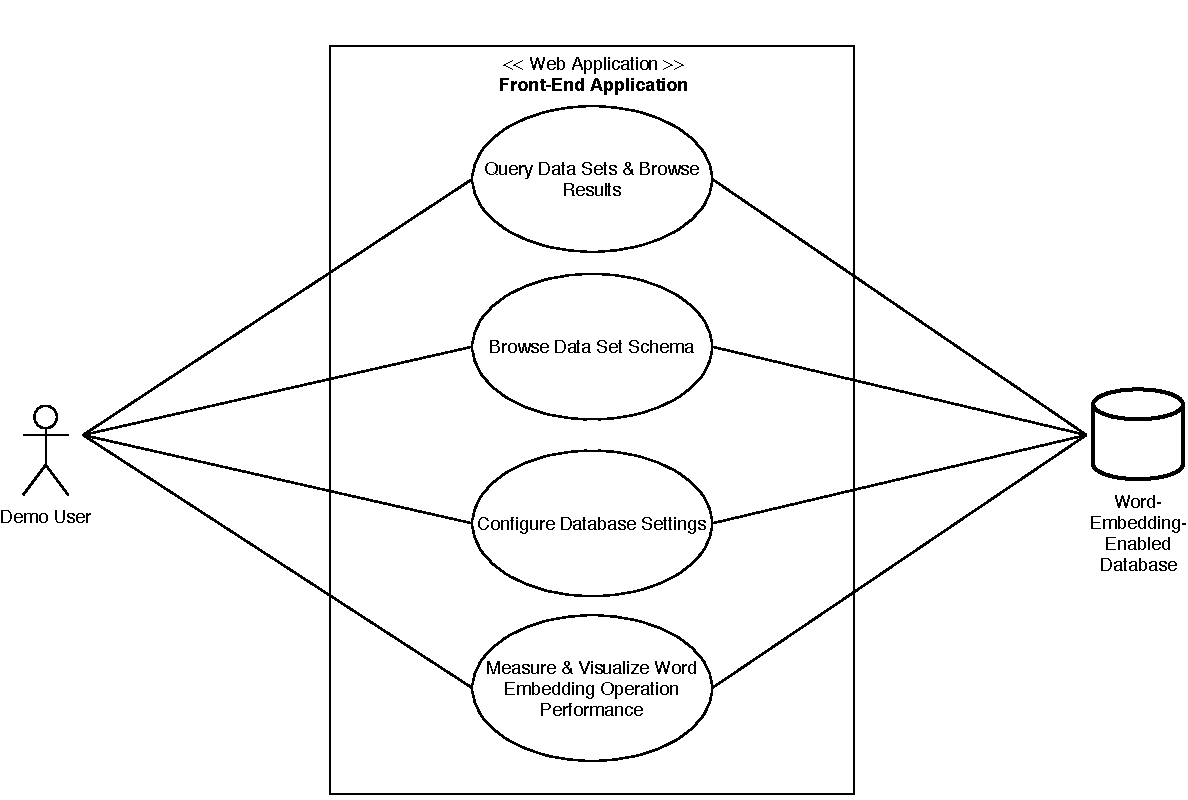
\includegraphics[width=\textwidth,keepaspectratio]{use_case_diagram.pdf}
	\caption{A diagram showing the use cases for the web application.}
	\label{fig:use_case_diagram}
\end{figure}

In Figure \ref{fig:use_case_diagram} above, the different use cases for the web application are shown as a UML use case diagram. There are two chief actors: the \textit{demo user} and the \textit{word-embedding enabled database}. The application developed in this thesis, here called the \textit{front-end application\footnote{\textit{"Front-end"} here is used relative to the database system. The web application's actual architecture comprises both a front end and a back end in the web development sense.}}, serves as an intermediary between them. The demo user interacts with the web application via a graphical web interface, while the web application is responsible for communicating with the database, sending queries to it and processing and presenting data received from it. The \textit{word-embedding enabled database} is where the different data sets (both the ones containing word embeddings and domain-specific ones) are stored and word embedding operations are executed.

Four main use cases for the web application have been identified, which I describe one by one:

\begin{enumerate}[label=U\arabic*]
	\item querying domain-specific data sets using word embedding operations and browsing query results;
	\item browsing the schema of the selected domain-specific data set;
	\item configuring the database's word-embedding-specific settings;
	\item measuring and visualizing a word embedding operation's performance.
\end{enumerate}

In the following descriptions of the use cases, it is assumed that both the web application and the database system are up and running and the user has loaded the web application using their browser.

\subsubsection{[U1] Query Data Sets and Browse Results}

A FREDDY system, just like any PostgreSQL system, is able to store arbitrary relational data sets, regardless of their specific domain. The web application should allow the user to execute word-embedding operations on textual data contained within them and present a query's results clearly. Figure \ref{fig:use_case_querying} shows a scenario for this use case.
\begin{figure}
	\centering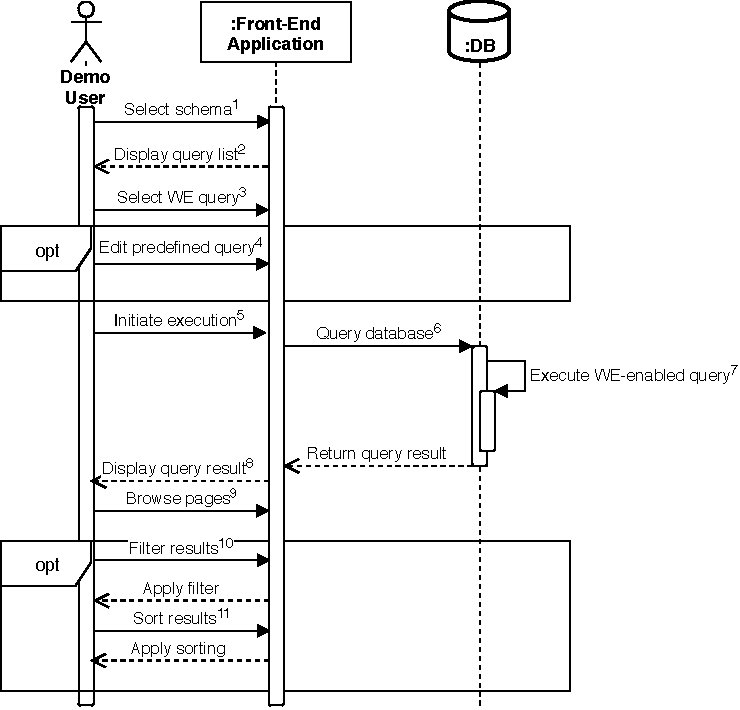
\includegraphics{sequence_use_case_querying.pdf}
	\caption{A sequence diagram for the use case of querying a word-embedding-enabled database.}
	\label{fig:use_case_querying}
\end{figure}
\begin{enumerate}
	\item The user selects the data set to be queried from a list of schemas.
	\item The web application automatically offers the user a list of predefined word-embedding-enabled queries relevant to the selected data set.
	\item The user selects a predefined query.
	\item \textit{Optionally, the user edits the predefined query according to their intent using a built-in text editor.}
	\item The user initiates the execution of the word-embedding enabled query.
	\item The web application sends the user-selected query to the word-embedding-enabled database system for execution.
	\item The database system executes the SQL query and returns its result to the web application.
	\item The web application displays the results graphically.
	\item The user browses the results, switching between different pages.
	\item \textit{Optionally, the user can filter the results by a keyword specified by them.}
	\item \textit{Again optionally, the user can sort the results by any column in ascending or descending alphanumerical order.}
\end{enumerate}

\subsubsection{[U2] Browse Data Set Schema}
While the web application should provide a list of predefined queries for each schema in the database, the user should also have the possibility to compose new queries on any chosen data set. To this end, the user should be able to obtain information about a data set's structure. Figure \ref{fig:use_case_schema} shows a scenario for this use case.
\begin{figure}
	\centering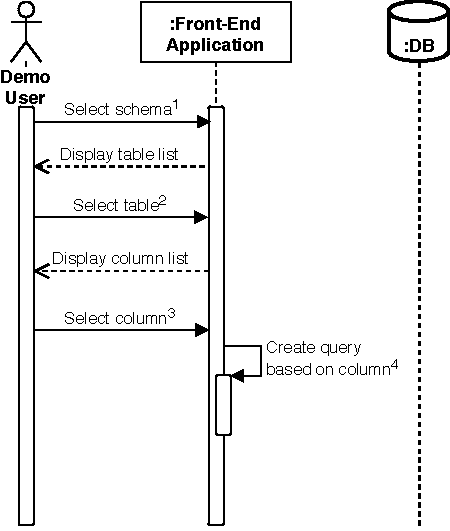
\includegraphics{sequence_use_case_schema.pdf}
	\caption{A sequence diagram for the use case of browsing a domain-specific data set's schema.}
	\label{fig:use_case_schema}
\end{figure}
\begin{enumerate}
	\item The user selects a data set from a list of schemas. The front-end application responds by displaying a list of tables in the selected data set.
	\item The user requires information about the properties of a specific table. The web application displays a list of columns in the table, including their data types.
	\item The user selects a column from the list.
	\item The web application automatically proposes to the user to send a query to list values of the specified column of the chosen table in order to give them a general idea about the column's contents.
\end{enumerate}

\subsubsection{[U3] Configure Database Settings}
The user should be able to alter the database's word-embedding-specific settings graphically using the front-end application at any time. The settings are then to be applied to all following word embedding operations executed from the front end. Figure \ref{fig:use_case_settings} shows a scenario for this use case.
\begin{figure}
	\centering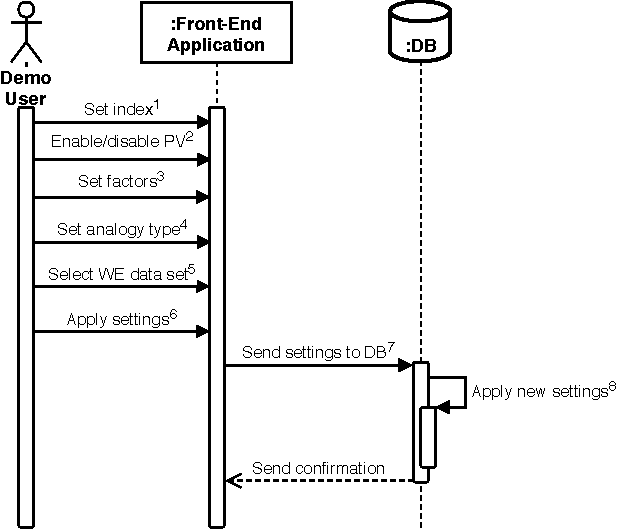
\includegraphics{sequence_use_case_settings.pdf}
	\caption{A sequence diagram for the use case of configuring the settings of a word-embedding-enabled database.}
	\label{fig:use_case_settings}
\end{figure}
\begin{enumerate}
	\item The user sets the index to be used for word embedding operations: no index (\textit{RAW}), PQ or IVFADC.
	\item The user enables or disables additional post-verification (if an index was selected in the previous step).
	\item The user sets index-dependent factors and the factor for post-verification.
	\item The user selects the analogy implementation to be used.
	\item The user selects a word embeddings data set to be used.
	\item The user requests the application of the selected settings.
	\item The front-end application sends the user-defined settings to the database system.
	\item The database system applies the selected settings and sends a confirmation to the web application.
\end{enumerate}

\subsubsection{[U4] Measure \& Visualize Word Embedding Operation Performance}
The web application should provide a way for the user to test FREDDY's word embedding operations' performance using various parameters and visualize the metrics of a performance test in its graphical user interface. Figure \ref{fig:use_case_performance} shows a scenario for this use case.
\begin{figure}
	\centering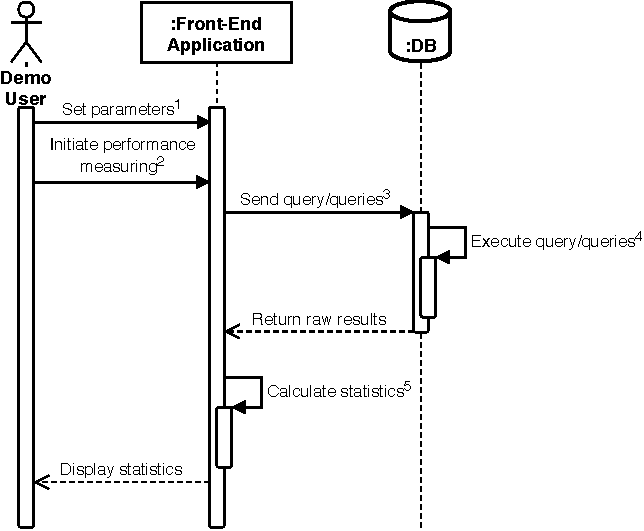
\includegraphics{sequence_use_case_performance.pdf}
	\caption{A sequence diagram for the use case of measuring a word embedding operation's performance.}
	\label{fig:use_case_performance}
\end{figure}
\begin{enumerate}
	\item The user sets the parameters for the performance test.
	\item The user requests the initiation of the performance test.
	\item The front end requests the execution of the specific queries constituting the performance test.
	\item The database executes the requested word embedding operations and returns their respective results and durations to the front end.
	\item The web application calculates the statistics of the operation's \textit{precision} and \textit{average execution time}.
	\item The front end displays the results of the performance test as a point on a chart with \textit{precision} and \textit{average execution time} as its axes.
\end{enumerate}
With each performance test executed, new points should be added to the chart. They should also be visually distinguishable according to the respective test's parameters and results.

\section{Example Scenario}
\label{sec:req_example_scenario}
\begin{figure}
	\centering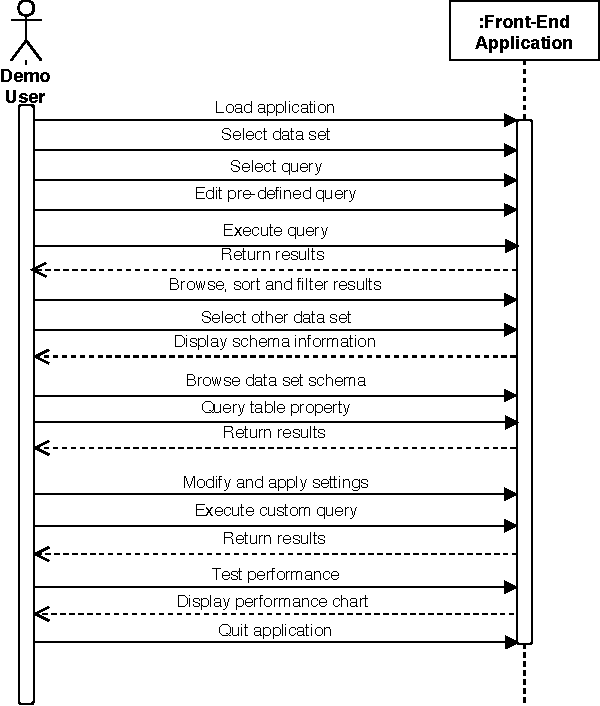
\includegraphics[width=0.6\textwidth, keepaspectratio]{sequence_example_scenario.pdf}
	\caption{A sequence diagram presenting an example scenario for the web application's use.}
	\label{fig:example_scenario}
\end{figure}
Figure \ref{fig:example_scenario} presents an example scenario of a complete user interaction with the web application, combining the previously described use cases. First, the user loads the web application using their browser. They select one of the provided domain-specific data sets and an example query for it. Using the built-in text editor, they edit the query according to their preferences. Afterwards, the query is executed and its results are shown to the user as a table. They switch between multiple pages of results, sort them according to a specific attribute and search for a keyword in the results. Then, the user selects another domain-specific data set. The web application shows a list of tables contained in it. The user uses the displayed list to find a specific property of a table they are looking for and sends a query for it. Then, the user alters the settings for used index, post-verification and used analogy implementation various and switches to another word embeddings data set. They enter a custom query into the text editor, execute it and examine the results. After that, the user decides to test FREDDY's k-NN search implementation's performance. They enter the desired parameters for the k-NN test and execute it. The web application conducts the requested test and displays a chart with its result. The user repeats the performance test with different indexes, post-verification and parameters. After examining the test results, the user decides that their interaction with the application is over and exits the application.

\section{Requirements}
\label{sec:requirements}
The requirements for the web application are divided into \textit{functional} and \textit{non-functional} requirements. The \textit{functional} requirements are derived from the use cases and example scenario described above and define the web application's functionality and behavior, while the \textit{non-functional} requirements elaborate its performance and usability characteristics.

\subsection{Functional Requirements}
\subsubsection{[R1] Requirements for use case U1: Query Data Sets and Browse Results}
\begin{enumerate}[label=R1.\arabic*]
	\item The web application should provide an option to switch between different domain-specific data sets stored in the database.
	\item A set of example predefined queries containing word embedding operations should be provided by default.
	\item The web application should provide a built-in, syntax-highlighted query editor for query customization.
	\item Initiating a query execution in the web application should result in the word-embedding enabled database executing the query and returning the query results to the front end.
	\item Query results should be shown in the front end as a table, with options for the user to sort and filter results. Furthermore, for the sake of better usability, the results should be split into multiple pages.
\end{enumerate}

\subsubsection{[R2] Requirements for use case U2: Browse Data Set Schema}
\begin{enumerate}[label=R2.\arabic*]
	\item After selecting a domain-specific data set, a list of tables contained within it should be displayed.
	\item The columns of each table and their data types should be shown explicitly.
	\item An option to display several values from a given column should be provided for a better overview over a table's contents by auto-filling the query editor with the respective projection query.
\end{enumerate}

\subsubsection{[R3] Requirements for use case U3: Configure Database Settings}
The web application should provide options to change the following FREDDY settings:
\begin{enumerate}[label=R3.\arabic*]
	\item index used;
	\item post-verification;
	\item index and post-verification factors;
	\item analogy function implementation;
	\item word embeddings data set used.
	\item Furthermore, settings should take effect immediately and for all following operations after their application.
\end{enumerate}

\subsubsection{[R4] Requirements for use case U4: Measure \& Visualize Word Embedding Operation Performance}
\begin{enumerate}[label=R4.\arabic*]
	\item There should be an option for the user to adjust the parameters for a performance test.
	\item The web application should calculate the measures of \textit{precision} and \textit{average execution time}.
	\item A performance test's results should be presented as a data point on a chart with the aforementioned measures as its axis.
	\item There should be a visual distinction between different tests' data points based on their parameters, index and post-verification used.
	\item Executing further performance tests should not result in the loss of previous data points.
\end{enumerate}

\subsection{Non-Functional Requirements}
\begin{enumerate}[label=N\arabic*]
	\item The application's graphical user interface should be designed according to modern design principles and ensure good usability and short response times.
	\item The web application's architecture should be split into multiple components in order to separate the presentation layer, application layer and the data access layer.
	\item The web application should not cause a large overhead for query execution: a query's execution time should depend chiefly on the database system's performance.
	\item The web application's front end should be compatible with modern web browsers.
\end{enumerate}

\subsubsection{Evaluating Non-Functional Requirements}
While the functional requirements can be evaluated by simply assessing the features of the completed web application, evaluating the non-functional requirements warrants additional examination. N1 is evaluated according to user experience design principles derived from psychological research \cite{laws-of-ux}. N2 is taken into consideration when choosing the technologies and architectural patterns used in the project's implementation. N3 is evaluated by conducting performance measurements on the database system and the web application. N4 is evaluated by testing the web application using two state-of-the-art web browsers. For further information about methods used in the evaluation of non-functional requirements and their results, see Section \ref{sec:nf_req}.